
\documentclass[14pt]{extbook}
%General Packages
\usepackage{multicol, enumerate, enumitem, hyperref, color, soul, setspace, parskip, fancyhdr}

%Math Packages
\usepackage{amssymb, amsthm, amsmath, bbm, latexsym, units, mathtools}

%All math in Display Style
\everymath{\displaystyle}

% Packages with additional options
%\usepackage[T1]{fontenc}
\usepackage[headsep=0.5cm,headheight=12pt, left=1 in,right= 1 in,top= 1 in,bottom= 1 in]{geometry}
\usepackage[usenames,dvipsnames]{xcolor}

% SageTeX
\usepackage{sagetex}

% Package to use the command below to create lines between items
\usepackage{dashrule}
\newcommand{\litem}[1]{\item#1\hspace*{-1cm}\rule{\textwidth}{0.4pt}}

\pagestyle{fancy}
\lhead{Module\,6\,-\,Polynomial\,Functions}
\chead{}
\rhead{Progress Exam 6}
\lfoot{Summer\,C\,2020}
\cfoot{}
\rfoot{Version B}

\begin{document}
\pagestyle{fancy}

\begin{sagesilent}
load("../Code/pythonImports.sage")
load("../Code/intervalMaskingMethod.sage")
load("../Code/keyGeneration.sage")
load("../Code/commonlyUsedFunctions.sage")
keyFileName = "Module6"
version = "B"
\end{sagesilent}

\begin{enumerate}
%\setcounter{enumi}{25}


\begin{sagesilent}
moduleNumber="6"
problemNumber=26
load("../Code/06polynomial/polyZeroBehavior.sage")
\end{sagesilent}

\litem{ \sage{displayStem}

\[ \sage{displayProblem} \]

\begin{enumerate}[label=\Alph*.]
    \begin{multicols}{2}
	      \item 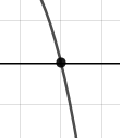
\includegraphics[width = 0.3\textwidth]{../Figures/polyZeroBehaviorAB.png}
		    \item 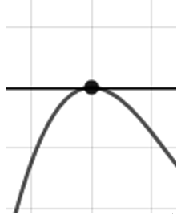
\includegraphics[width = 0.3\textwidth]{../Figures/polyZeroBehaviorBB.png}
		    \item 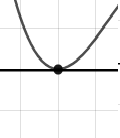
\includegraphics[width = 0.3\textwidth]{../Figures/polyZeroBehaviorCB.png}
		    \item 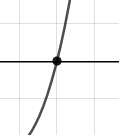
\includegraphics[width = 0.3\textwidth]{../Figures/polyZeroBehaviorDB.png}
    \end{multicols}
        \item \text{None of the above.}
\end{enumerate}
}

  \begin{sagesilent}
  moduleNumber="6"
  problemNumber=27
  load("../Code/06polynomial/polyGraphToFunction.sage")
  \end{sagesilent}

  \litem{ \sage{displayStem}

   \begin{center}
       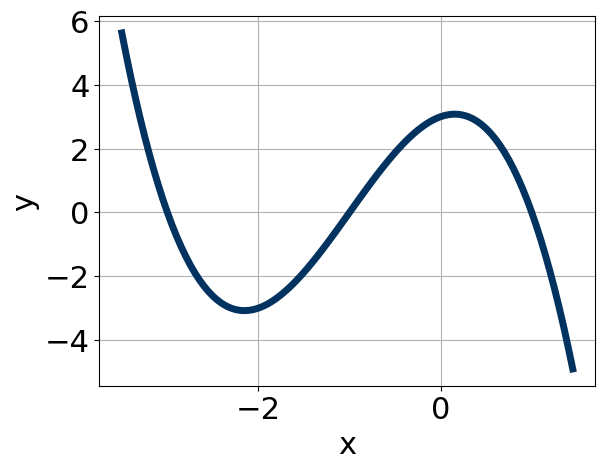
\includegraphics[width=0.5\textwidth]{../Figures/polyGraphToFunctionB.png}
   \end{center}

  	\begin{enumerate}[label=\Alph*.]
    \item \( \sage{choices[0]} \)
    \item \( \sage{choices[1]} \)
    \item \( \sage{choices[2]} \)
    \item \( \sage{choices[3]} \)
    \item \( \sage{choices[4]} \)
  	\end{enumerate}
  }

\begin{sagesilent}
moduleNumber="6"
problemNumber=28
load("../Code/06polynomial/polyEndBehavior.sage")
\end{sagesilent}

\litem{ \sage{displayStem}

\[ \sage{displayProblem} \]

\begin{enumerate}[label=\Alph*.]
    \begin{multicols}{2}
	      \item 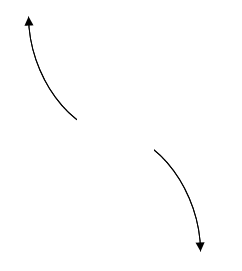
\includegraphics[width = 0.3\textwidth]{../Figures/polyEndBehaviorAB.png}
		    \item 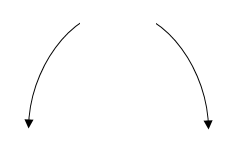
\includegraphics[width = 0.3\textwidth]{../Figures/polyEndBehaviorBB.png}
		    \item 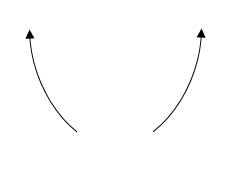
\includegraphics[width = 0.3\textwidth]{../Figures/polyEndBehaviorCB.png}
		    \item 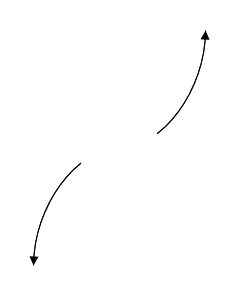
\includegraphics[width = 0.3\textwidth]{../Figures/polyEndBehaviorDB.png}
    \end{multicols}
        \item \text{None of the above.}
\end{enumerate}
}
\begin{sagesilent}
moduleNumber="6"
problemNumber=29
load("../Code/06polynomial/constructPolyRationals.sage")
\end{sagesilent}

\litem{ \sage{displayStem}

   \[ \sage{displayProblem} \]

  	\begin{enumerate}[label=\Alph*.]
    \item \( \sage{choices[0]} \)
    \item \( \sage{choices[1]} \)
    \item \( \sage{choices[2]} \)
    \item \( \sage{choices[3]} \)
    \item \( \sage{choices[4]} \)
  	\end{enumerate}
  }
\begin{sagesilent}
moduleNumber="6"
problemNumber=30
load("../Code/06polynomial/constructPolyComplex.sage")
\end{sagesilent}

\litem{ \sage{displayStem}

   \[ \sage{displayProblem} \]

  	\begin{enumerate}[label=\Alph*.]
    \item \( \sage{choices[0]} \)
    \item \( \sage{choices[1]} \)
    \item \( \sage{choices[2]} \)
    \item \( \sage{choices[3]} \)
    \item \( \sage{choices[4]} \)
  	\end{enumerate}
  }

\end{enumerate}

\end{document}

